%%%%%%%%%%%%%%%%%%%%%%%%%%%%%%%%%%%%%%%%%%%%%%%%%%%%%%%%%%%%%%%%%%%%%%%%%%%%%%%
%%% Describe how the wave solution comes about for Einstein's eqns in vacuum, 
%%% and discuss the two-body problem at leading order.
%%%%%%%%%%%%%%%%%%%%%%%%%%%%%%%%%%%%%%%%%%%%%%%%%%%%%%%%%%%%%%%%%%%%%%%%%%%%%%%

\newcommand{\cd}{\nabla}
\newcommand{\pd}{\partial}
\newcommand{\Reals}{\mathcal{R}}
\newcommand{\defeq}{\mathrel{\mathop:}=}
\newcommand{\hbarr}{\bar{h}}
\newcommand{\Tbar}{\bar{T}}
\newcommand{\Quad}{\mathcal{Q}}
\newcommand{\vecx}{\mathbf{x}}
\newcommand{\vecr}{\mathbf{r}}

In this chapter we briefly review the treatment of compact object
binaries in General Relativity (henceforth GR), with a view at providing a 
description of the gravitational waves emitted during their coalescence. 
% In Sec.~\ref{sec:general_relativity}, we revise the basic concepts of 
% differential geometry and their application in general relativity. 
% Then we go on to describe the generation of gravitational radiation in 
% linearized GR in Sec.~\ref{sec:gravitational_radiation}. 
% In Sec.~\ref{sec:effects_of_waves}, we describe the effect of incident
% gravitational waves on freely-falling particles. This discussion will 
% be carried over in the next chapter where we discuss the concept
% and design of interferometric gravitational wave detectors. 
% In Sec.~\ref{sec:PNWaveforms} we discuss the generation of gravitational waves
% by a compact object binary system in quasi-circular orbits, as it evolves 
% through the inspiral phase to its coalescence. 
Searches performed over 
detector data use theoretically modeled waveforms for compact binaries as 
filters. We briefly summarize two of the primary waveform models applicable
to LIGO-Virgo sources in Sec.~\ref{sec:PNWaveforms}.


% \section{General Relativity}
% \label{sec:general_relativity}
% 
% We begin with summarizing basic concepts of differential geometry used 
% and work up to writing down Einstein's equations. Readers are referred
% to the books by Misner, Thorne and Wheeler~\cite{mtw}, 
% Schutz~\cite{BSchutzBook}, and Wald~\cite{WaldBook} for broader treatments
% of these topics.
% 
% \subsection{Manifolds: Vectors, Forms and Tensors}
% 
% An manifold is a set that has the local differential 
% structure of $\Reals^n$, but not necessarily its global properties. 
% An n-dimensional, infinitely continuously differentiably (i.e. $C^\infty$
% real manifold $M$ is a set along with sub-sets $S_\alpha$, which together
% obey the following
% properties:
% \begin{enumerate}
%  \item Every element $p\in M$, is a member of at least one $S_\alpha$.
%  This ensures that $\{S_\alpha\}$ covers M.
%  \item There exists a one-to-one, onto, map $\Psi_\alpha :S_\alpha \rightarrow U_\alpha$
%  for each subset $S_\alpha$ to an open subset of $\Reals^n$, $U_\alpha$. This ensures
%  that locally, every {\it patch} of the manifold $M$ has the properties of 
%  a Euclidian space.
%  \item If any two subsets $S_\alpha$ and $S_\beta$ overlap, there exists a $C_\infty$
%  map $\zeta\defeq\Psi_\beta \circ \Psi_\alpha^{-1}$ which maps elements of the open 
%  set $U_\alpha \subset \Reals^n$ to $U_\beta \subset \Reals^n$ (with notation as
%  above). 
% \end{enumerate}
% {\it Curves} are maps from $\Reals^n$ to the manifold $M$, 
% and {\it scalar functions} are reverse maps from $M\rightarrow \Reals^n$. 
% A composite of a function $f$ with a curve $\gamma$ gives a map from
% $\Reals^n\rightarrow\Reals^n$. 
% %
% Doing calculus on manifolds invokes the concept of 
% {\it vectors} in a local sense, or {\it tangent} vectors.
% In general, there is no concept of vector operations over vectors at 
% different poins in the manifold, as there is in vector spaces. 
% A tangent vector $u$ at a point $p\in M$ is defined as a
% linear differentiation operator which maps functions defined at $p$,
% to $\Reals$. By definition, $u$ obeys the Leibnitz rule:
% \begin{equation}\nonumber
%  u(f(p) g(p)) = u(f(p)) g(p) + f(p) u(g(p)) 
% \end{equation}
% where both $f$ and $g$ are functions in the sense mentioned above.
% The tangent vectors exist in a {\it distinct} n-dimensional vector space $T_pM$
% at each point $p$ in the manifold. 
% They can be identified with local directional derivatives
% and be decomposed in the local coordinate basis $\pd/\pd x^\mu$,
% where $\{x^\mu\}$ forms the coordinate system on $\Reals^n$.
% We will denote this special basis as $\pd_\mu$ or $\vec{e}_\mu$ henceforth.
% A tangent vector field can be defined over the manifold, associating each point 
% $p\in M$ to a vector defined locally at $p$.
%  
% \iffalse
% \begin{equation*}
% \frac{d}{d \lambda} fi \big|_p = 
%   \frac{d}{d\lambda} (f \circ \gamma) \big|_p
% \end{equation*}
% 
% 
% Expanding this in terms of a chart whose domain includes $p$ and then
% applying the chain rule
%  
% \begin{align*}
% \frac{d}{d \lambda} fi \big|_p &= 
%  \frac{d}{d\lambda} ( (f \circ \phi^{-1}) \circ (\phi \circ
% \lambda) ) \\
% &= \frac{d(\phi^{-1} \circ \gamma)^\mu}{d\lambda} 
% \frac{\partial (f \circ \phi^{-1}) }{\partial x^\mu} \big|_p \\
% &= \frac{dx^\mu}{d\lambda} \partial_\mu f \big|_p
% \end{align*}
% 
% where $x^\mu$ are the coordinates on $\mathcal{R}^n$.  Finally, since
% the function $f$ is arbitrary we can define
% 
% \begin{equation}
% \label{eq:tangent_vector}
% \frac{d}{d\lambda} = \frac{dx^\mu}{d\lambda} \partial_\mu
% \end{equation}
% \fi
% 
% A \emph{one-form} (or a {\it dual} vector) is a linear map from vectors to
% $\Reals$, e.g. for a point $p\in M$, $\omega :T_pM\rightarrow\Reals$. 
% The set of one-forms at the point $p$ form a vector space. A natural basis
% for the same, $\{\tilde{\omega}^\mu\}$, can be obtained by solving
% %
% \begin{equation*}
% \tilde{\omega}^\nu \vec{e}_\mu = \delta_\mu^\nu
% \end{equation*}
% %
% The components of an arbitrary form $\omega$ in this basis may be
% found by the application of the form to basis vectors, i.e.
% $\omega_\mu\defeq \omega(\vec{e}_\mu)$.
% %
% \iffalse
% \begin{align*}
% \omega(\vec{e}_\nu)
% &= \tilde{\omega}^\mu \omega_\mu (\vec{e}_\nu) \\
% &= \omega_\mu \tilde{\omega}^\mu (\vec{e}_\nu) \\
% &= \omega_\mu \delta^\nu_\mu \\
% &= \omega_\nu\\
% \end{align*}
% \fi
% %
% From vectors and one-forms, we can build up an arbitrary ${m \choose n}$
% {\it tensor} as a linear map from outer products of $m$ vectors and $n$ 
% one-forms to $\mathcal{R}$.  The components of a tensor $T$ in a choice of
% coordinates can be found by applying it to combinations of the basis
% vectors and basis one-forms.  Finally, a ${m \choose n}$ tensor field is
% a map that associates to each point $p$ in $\mathcal{M}$ an element in
% the space of  ${m \choose n}$ tensors at $p$.
% 
% \subsection{The Metric Tensor}
% 
% Over the 4-dimensional manifold of spacetime, we can define a metric $g$
% which is a ${2\choose 0}$ tensor with the following properties:
% \begin{itemize}
%  \item It defines the notion of a distance between infinitesimally separated 
%  points $ds$, 
%  \begin{equation}
%   ds^2\defeq g_{\mu\nu} dx^\mu dx^\nu.
%  \end{equation}
%  \item It is symmetric in its indices, i.e. $g_{\mu\nu}=g_{\nu\mu}$.
%  \item The determinant $|g_{\mu\nu}|$ is non-zero, making $g$ invertible: 
%  $\exists\, g^{\rho\nu}: g_{\mu\rho}g^{\rho\nu} = \delta^\nu_\mu$.
% %  \item 
% \end{itemize}
% % 
% % 
% % A particularly important tensor in general relativity is the
% % \emph{metric}, a ${2 \choose 0}$ tensor that is symmetric ($g_{\mu\nu}
% % = g_{\nu\mu})$ and non-degenerate (the determinant of $g$ taken as a
% % matrix $|g_{\mu\nu}| \neq 0$.  The latter feature makes it possible to
% % define the inverse metric $g^{\mu\nu}$ as
% % %
% % \begin{equation*} g^{\mu_\rho} g_{\rho_\nu} = \delta^\mu_\nu
% % \end{equation*}
% % %
% Given a vector $x^\mu$ the object $g_{\mu\nu} x^\mu$ maps another
% vector to a real number, and is therefore a one-form.  The metric
% therefore maps between the space of vectors and the space of 
% one-forms.  
% % Most importantly, the metric defines a notion of
% % distance on the manifold.  Infinitesimally
% % %
% % \begin{equation} ds^2 = g_{\mu\nu} dx^\mu dx^\nu \end{equation}
% % %
% In special relativity, in Cartesian coordinates, the metric has
% components $(-1,1,1,1)$ along the diagonal, and all other components are
% zero. This {\it flat} spacetime metric will be denoted $\eta_{\mu\nu}$
% henceforth.
% 
% \subsection{Covariant Derivative and Parallel Transport}
% \label{ssec:covariant_derivative}\label{ssec:parallel}
% 
% A {\it (covariant) derivative operator} $\cd$ on a manifold $M$ is a map
% which takes each differentiable ${m\choose n}$ tensor field to a smooth
% tensor field of type ${m\choose n+1}$, and satisfies the following properties:
% \begin{itemize}
%  \item Linearity: $\cd_\alpha (kA^{a_1\dots a_m}_{b_1\dots b_n} + lB^{a_1\dots a_m}_{b_1\dots b_n}) = k\cd_\alpha A^{a_1\dots a_m}_{b_1\dots b_n} + l\cd_\alpha B^{a_1\dots a_m}_{b_1\dots b_n}$,
%  \item Leibnitz rule: $\cd_\alpha (A^{a_1\dots a_m}_{b_1\dots b_n} B^{a_1\dots a_m}_{b_1\dots b_n}) = \cd_\alpha (A^{a_1\dots a_m}_{b_1\dots b_n}) B^{a_1\dots a_m}_{b_1\dots b_n} + A^{a_1\dots a_m}_{b_1\dots b_n} \cd_\alpha (B^{a_1\dots a_m}_{b_1\dots b_n})$,
%  \item Commutativity with contraction of indices:  $\cd_\alpha (A^{a_1\dots c\dots a_m}_{b_1\dots c\dots b_n}) = \cd_\alpha A^{a_1\dots c\dots a_m}_{b_1\dots c\dots b_n}$, and, 
%  \item Agrees with the notion of tangent vectors as directional derivatives on scalar fields.%: $v(f) = v^\alpha\cd_\alpha f$. 
% \end{itemize}
% In GR, it is additionally required that the commutator of the derivative 
% operator $[\cd_\alpha, \cd_\beta]f\defeq [\cd_\alpha\cd_\beta - \cd_\beta\cd_\alpha]f$ 
% be zero when acting on a scalar field $f:M\rightarrow\Reals$, 
% a condition that has so far been borne by experiments.
% This commutator is called the {\it torsion} tensor, and $\cd$ is called
% {\it torsion} free if the above condition is satisfied.
% 
% The application of $\cd$ on a vector field gives
% %
% \begin{equation}
%  \cd_\mu x^{\nu} \vec{e}_\nu = \cd_\mu (x^\nu) \vec{e}_\nu + x^\nu \cd_\mu \vec{e}_\nu,
% \end{equation}
% %
% where the second term on the right may not vanish in coordinate systems 
% other than Cartesian in flat spacetime, or in curved spacetime. However, 
% we must be able to write the new vector in the original basis. The components
% are called {\it connection coefficients}, and are denoted as $\Gamma^\rho_{\mu\nu}$:
% %
% \begin{align}\label{eq:covariant_derivative}
%  \cd_\mu x^{\nu} \vec{e}_\nu &= \cd_\mu (x^\nu) \vec{e}_\nu + x^\nu \Gamma^\rho_{\nu\mu} \vec{e}_\rho \\
%  &= (\pd_\mu x^\nu + x^\rho \Gamma^\nu_{\rho\mu}) \vec{e}_\nu
% \end{align}
% In similar notation, the action of $\cd$ on a one-form $\omega$ can be obtained, 
% noting that $\cd_\mu (v^\nu \omega_\nu) = \pd_\mu (v^\nu \omega_\nu)$, such that
% %
% \begin{equation}
%  \cd_\mu \omega_\nu = \pd_\mu\omega_\nu + \Gamma^\rho_{\mu\nu}\omega_\rho.
% \end{equation}
% Extending this to general ${m\choose n}$ tensors, we get that 
% \begin{equation}
%  \cd_\mu T^{a_1\dots a_m}_{b_1\dots b_n} = \pd_\mu T^{a_1\dots a_m}_{b_1\dots b_n} + \Sum_{i} \Gamma^{a_i}_{\mu d} T^{a_1\dots a_{i-1} d\dots a_m}_{b_1\dots b_n} - \Sum_{i} \Gamma^{d}_{\mu b_i} T^{a_1\dots a_m}_{b_1\dots b_{i-1} d\dots b_n}.
% \end{equation}
% 
% The covariant derivative gives differential structure to the manifold $M$, 
% allowing for moving a vector {\it without changing it}, or in other words
% the ``parallel transport'' of a vector. Given the operator $\cd_\alpha$, a vector 
% $v$ is said to be parallel transported along a curve $C$, with a tangent 
% vector $t^\alpha$, if 
% \begin{equation}\label{eq:parallel_transport}
%  t^\alpha \cd_\alpha v^\beta = 0
% \end{equation}
% all along $C$. An intuitive visualization of parallel transport is of 
% moving a vector that is perpendicular to the Equator of the Earth (at longitude
% $L_0$) parallel to itself along the Equator, followed by transporting it along
% a different longitude $L_1$ till it reaches the North pole, and further
% parallel transporting it back along $L_0$ to its original location.
% The returned vector would not be parallel to the original vector, even 
% though it was never rotated with respect to itself. This therefore 
% indicates that the surface on which it was moved is itself curved.
% Eq.~\ref{eq:parallel_transport} shows that the parallel transport 
% of $v^\alpha$ depends solely on itself along the curve $C$. Also, 
% it can be shown that given an initial value of $v^\alpha$,
% Eq.~\ref{eq:parallel_transport} always has a unique solution~\cite{WaldBook}. 
% A remarkable result follows, which is that a vector at a point $p$ on the curve
% $C$ uniquely defines a ``parallel transported vector'' everywhere else on $C$.
% This idea will also help us define curvature in a later section of this 
% chapter.
% 
% Of particular interest is the case where a vector is
% parallel-transported along itself
% %
% \begin{equation*}
% v^\mu \nabla_\mu v^\nu = v^\mu (\partial_\mu v^\nu + \Gamma^\nu_{\mu\rho} v^\rho) = 0.
% \end{equation*}
% %
% Now consider a curve $x(\lambda)$ such that $v$ is the tangent to this
% curve, $v^\mu = d x^\mu/d\lambda$, then
% %
% \begin{align}
% \label{eq:geodesic}
% \frac{d x^\mu}{d\lambda}
%   \frac{\partial }{\partial x^\mu}
%   \frac{d x^\nu}{d\lambda}  
% + \Gamma^\nu_{\mu\rho} 
% \frac{d x^\mu}{d\lambda}
% \frac{d x^\rho}{d\lambda} &= 0 \nonumber \\
% \frac{d^2 x^\nu}{d\lambda^2}
% + \Gamma^\nu_{\mu\rho} 
% \frac{d x^\mu}{d\lambda}
% \frac{d x^\rho}{d\lambda} &= 0 
% \end{align}
% %
% Eq.~\ref{eq:geodesic} is called the the \emph{geodesic equation}. 
% The solution to this equation defines the path along which test masses 
% that are acting solely under the influence of gravity move, in other 
% words it defines the trajectory of freely falling particles. 
% 
% \subsection{The Christoffel Symbols}
% 
% Given just the manifold structure, many distinct derivatives can be 
% defined on it. However, with the availability of a metric $g_{\mu\nu}$, 
% we can require another condition that scalars do not change 
% under parallel transport along an arbitrary vector $t^\alpha$. 
% For arbitrary vector fields $u^\alpha$ and $v^\beta$, we take the 
% scalar $g_{\mu\nu}u^\mu v^\nu$ and require that
% %
% \begin{align}\label{eq:parallel_transport_scalar}
% t^\mu \nabla_\mu (g_{\alpha\beta} u^\alpha v^\beta) = 0 =
% x^\mu (\nabla_\mu g_{\alpha\beta}) u^\alpha v^\beta
% + g^{\alpha\beta} (x^\mu \nabla_\mu u^\alpha) v^\beta
% + g^{\alpha\beta} u^\alpha (x^\mu \nabla_\mu v^\beta).
% \end{align}
% %
% As this must hold for arbitrary $u$ and $v$, it must also hold when
% both are constant. This sets the last two terms on the right hand side
% of Eq.~\ref{eq:parallel_transport_scalar} to zero. We have left
% %
% \begin{equation}
% \label{eq:metric_compatibility}
% \nabla_\mu g_{\alpha\beta} = 0,
% \end{equation}
% which is also known as the {\it metric compatibility} condition. 
% 
% Equation~\ref{eq:metric_compatibility} and the requirement that $\cd$ be
% torsion-free together fix the connection coefficients $\Gamma$, which can be
% written in terms of the metric as:
% %
% \begin{equation}
% \Gamma^{\rho}_{\mu\nu}
% = \frac{1}{2} g^{\rho\sigma}\left[
% \partial_\nu g_{\mu\sigma}
% + \partial_\mu g_{\nu\sigma}
% - \partial_\sigma g_{\mu\nu}
% \right]
% \end{equation}
% % 
% Combining this with Eq.~\ref{eq:geodesic} in the previous section,
% we see that the motion of particles are completely specified once we know
% the metric of the spacetime and their initial positions and velocities.
% 
% \subsection{Field Equations of Gravity}
% 
% When a vector is parallel transported from a point $p$ to $q$ along $C$ in the
% manifold $M$, the final vector at $q$ will, in general, depend on the choice of
% $C$. We can generalize the example given in Sec.~\ref{ssec:covariant_derivative}
% and use the path dependence of parallel transport to define an instrinsic notion
% of curvature of the underlying manifold. We transport a vector $u^\alpha$ along
% an infinitesimal parallelogram with sides defined by $v^\beta$ and $w^\gamma$.
% The failure of a vector to return to its original value when parallel 
% transported about a closed loop can be used to define the Riemann tensor
% $R^\rho_{\sigma\mu\nu}$:
% % 
% % 
% % We now generalize the example given in Sec.~\ref{ssec:covariant_derivative},
% % and ask how a vector $A^\mu$ changes as it is parallel-transported around
% % an infinitesimal parallelogram with sides defined by the vectors
% % $B^\mu$ and $C^\nu$.  Recalling that vectors and directional
% % derivatives are the same thing, it can be shown that this is
% % equivalent to asking how covariant derivatives fail to commute.  The
% % result must be linear in $A^\mu$ and so we may write
% %
% \begin{equation}
% \label{eq:riemann_def}
% \left[\nabla_\mu \nabla_\nu - \nabla_\nu \nabla_\mu\right] v^\rho
% = R^\rho_{\sigma\mu\nu} v^\sigma
% \end{equation}
% %
% A number of properties follow from this definition (which are either
% follow trivially or may be proven by substituting the definition of the
% covariant derivative, Eq.~\ref{eq:covariant_derivative}.  First, we note that
% $R^\rho_{\sigma\mu\nu}$ is (anti-)symmetric in the first and last pair of 
% its indices:
% %
% \begin{equation}
% \label{eq:symmetries}
% R_{\rho\sigma\mu\nu}
% = -R_{\sigma\rho\mu\nu}
% = -R_{\rho\sigma\nu\mu}
% = R_{\mu\nu\rho\sigma}
% \end{equation}
% %
% which also imply
% %
% \begin{align}
% R^\rho_{[\sigma\mu\nu]} = 0,
% \end{align}
% where $[\dots]$ denotes the anti-symmetrization over the enclosed indices.
% Second, we have the Bianchi identities,
% %
% \begin{equation}
% \label{eq:bianchi}
% \cd_\alpha R_{\rho\sigma\mu\nu}
% +\cd_\mu R_{\rho\sigma\nu\alpha}
% +\cd_\nu R_{\rho\sigma\alpha\mu} = 0
% \end{equation}
% 
% Eq.~\ref{eq:riemann_def} can be straightforwardly generalized to obtain 
% the change in an arbitrary tensor upon being parallel-transported around an
% infinitesimal loop.  It can be shown that~\cite{WaldBook}
% %
% \begin{equation}
% \label{eq:higher_order_riemann}
% \left[\nabla_\mu \nabla_\nu - \nabla_\nu \nabla_\mu\right] 
% B^{\rho_1 \rho_2 \ldots \rho_n}
% = - R^{\rho_1}_{\sigma \mu\nu} B^{\sigma \rho_2 \ldots \rho_n}
% - R^{\rho_2}_{\sigma \mu\nu} B^{\rho_1 \sigma \ldots \rho_n}
% - \ldots -
% - R^{\rho_n}_{\sigma \mu\nu} B^{\rho_1 \rho_2 \ldots \sigma }
% \end{equation}
% %
% which can be proved by expanding
% %
% \begin{equation*}
% \left[\nabla_\mu \nabla_\nu - \nabla_\nu \nabla_\mu\right] 
% (\vec{e}_\rho \otimes \vec{e}_\sigma)
% \end{equation*}
% %
% and subsequently using the second principle of mathematical induction.  
% 
% Due to the symmetries of the Riemann tensor, it can be shown that there is 
% exactly one non-trivial contraction, up to a sign, which is between its
% first and third or second and fourth indices:
% %
% \begin{equation}
% R_{\mu\nu} = R^\sigma_{\mu\sigma\nu}.
% \end{equation}
% %
% $R_{\mu\nu}$ is also known as the {\it Ricci} tensor. Contracting again, we get
% %
% \begin{equation}
% R = R^\mu_\mu
% \end{equation}
% %
% which is the unique non-trivial \emph{Ricci} scalar that can be formed from
% the Riemann tensor.
% 
% Contracting the Bianchi identity twice gives
% %
% \begin{equation*}
% \cd_\alpha R_{\sigma\mu\nu}^\alpha + \cd_\sigma R_{\mu\nu} - \cd_\mu R_{\sigma\nu} = 0.
% \end{equation*}
% %
% Raising the index $\nu$ and contracting over $\mu$ and $\nu$, we obtain
% %
% \begin{equation*}
% \cd_\alpha R^\alpha_\mu + \cd_\sigma R_\mu^\sigma - \cd_\mu R = 0
% \end{equation*}
% %
% Relabeling the dummy indices and using metric compatibility gives
% %
% \begin{equation*}
% 2\cd^\mu \left(R_{\mu\nu} - \frac{1}{2} g_{\mu\nu} R \right) = 0,
% \end{equation*}
% %
% which defines the divergenceless tensor $G_{\mu\nu}$:
% %
% \begin{equation}
% \label{eq:einstein_tensor}
% G_{\mu\nu} = R_{\mu\nu} - \frac{1}{2} g_{\mu\nu} R
% \end{equation}
% %
% It follows trivially that $G$ is symmetric: $G_{\mu\nu} = G_{\nu\mu}$.
% 
% Continuous matter distributions in special relativity are described by a 
% symmetric tensor $T_{\mu\nu}$ called the {\it stress-energy-momentum} tensor.
% For an observer with 4-velocity $u^\mu$, the component $T_{\mu\nu}u^\mu u^\nu$
% is the energy density as measured by the observer. For non-relativistic matter,
% the energy density $\simeq T^{00}$ and is the same as the mass density $\rho$;
% while $T^{0i}$ is the momentum in the $i-$th direction. Conservation of 
% momentum, i.e. $\pd_t \rho = \pd_i p^i$ can therefore be written as
% % 
% % We now relate this to physics by noting that the matter and energy
% % content of a region is described by the stress-energy tensor
% % $T_{\mu\nu}$ where each component is ``the flow of $\mu$ momentum in the
% % $\nu$ direction.''  For example, the $0,0$ component is energy density
% % and the $0,i$ components are the $i^\mathrm{th}$ components of
% % momentum.
% % 
% % Conservation of energy requires that the difference in momentum
% % ($p^i$) across each face of a cube be balanced by a change of energy
% % ($\rho$), within the cube,
% % %
% % \begin{equation*}
% % \partial_t \rho = \partial_i p^i
% % \end{equation*}
% %
% % In terms of the stress-energy tensor this becomes
% %
% \begin{equation*}
% - \nabla^0 T_{00} + \nabla^i T_{0i} = \nabla^\nu T_{0 \nu} = 0
% \end{equation*}
% %
% However, as the time direction is not uniquely specified, a change of
% coordinates will mix space and time components. Therefore, the above
% equation must generalize to 
% %
% \begin{equation*}
% \nabla^\nu T_{\mu\nu} = 0,
% \end{equation*}
% %
% which says that the stress-energy-momentum tensor $T$ is divergenceless like
% $G$, and like $G$ it is also symmetric. Einstein proposed the ansatz
% %
% \begin{equation*}
% G_{\mu\nu} \propto T_{\mu\nu},
% \end{equation*}
% %
% where the proportionality constant is fixed by requiring agreement with 
% Newton's law of gravity in the low energy limit, when $T^{00}\gg$ all other
% components of $T$, to $8\pi$. Now, we can finally write down the field 
% equations of gravity which Einstein proposed in $1915$:
% %
% \begin{equation}
% \label{eq:einsteins_equation}
% G_{\mu\nu} = 8\pi T_{\mu\nu}
% \end{equation}
% %
% As $G_{\mu\nu}$ is entirely determined by the spacetime metric, and 
% the tensor $T$ is determined by the stresses, energy and momentum 
% distribution and flows of matter in the universe, these equations connect 
% the curvature of spacetime with properties of matter that resides in it.


% \section{Gravitational Radiation}
% \label{sec:gravitational_radiation}
% 
% Due to the nonlinear nature of the gravitational field equations, 
% Eq.~\ref{eq:einsteins_equation}, it is difficult to find its solutions, 
% and only a handful of exact solutions are known. However, solving them
% in the weak field approximation is often useful, mainly because the 
% gravitational fields encountered in many physical systems are indeed weak.
% A weak gravitational field is characterized by a metric of the form
% \begin{equation}\label{eq:metric_weak_field}
%  g_{\mu\nu} = \eta_{\mu\nu} + h_{\mu\nu}
% \end{equation}
% with $|h_{\mu\nu}|\ll 1$. In this approximation, we can think of the 
% spacetime as flat with $h_{\mu\nu}$ representing a ${2\choose 0}$ tensor
% field propagating on it. To linear order in $h_{\mu\nu}$ the Riemann 
% tensor can be found to be:
% \begin{equation}\label{eq:riemann_h_linear}
%  R^\alpha_{\beta\gamma\delta} = \frac{1}{2}\left(\pd_\gamma\pd_\beta h^\alpha_\delta + 
%  \pd_\delta\pd^\alpha h_{\beta\gamma} -
%  \pd_\gamma\pd^\alpha h_{\beta\delta} - 
%  \pd_\delta\pd_\beta h^\alpha_\gamma\right).
% \end{equation}
% Contracting on two of the indices, we can write the Ricci tensor to be:
% \begin{equation}
%  R_{\alpha\beta} = -\frac{1}{2}\left(\pd_\alpha\pd_\beta h + \Box h_{\alpha\beta} - 
%  \pd_\beta\pd_\gamma h^\gamma_\alpha - \pd_\gamma\pd_\alpha h^\gamma_\beta \right).
% \end{equation}
% With some algebric manipulation, and substituting 
% $h_{\mu\nu}\rightarrow \hbarr_{\mu\nu} = h_{\mu\nu} - \frac{1}{2}\eta_{\mu\nu}h$,
% the field equations reduce to
% \begin{equation}
%  \Box \hbarr_{\mu\nu} + \eta_{\mu\nu}\pd_\alpha\pd_\beta \hbarr^{\alpha\beta} - 
%  \pd_\nu\pd_\alpha \hbarr^\alpha_\mu - \pd_\mu\pd_\alpha\hbarr^\alpha_\nu = -16\pi T_{\mu\nu}.
% \end{equation}
% It can be shown that this equation is invariant under the gauge transformations
% produced by a vector $\zeta_\alpha$: 
% \begin{equation}\label{eq:h_gauge_transform1}
%  \hbarr^{\mu\nu} \rightarrow \hbarr^{'\mu\nu} = \hbarr^{\mu\nu} - 
%  \pd^\mu\zeta^\nu - \pd^\nu\zeta^\mu + \eta^{\mu\nu}\pd_\alpha \zeta^\alpha .
% \end{equation}
% Imposing the following gauge conditions
% \begin{equation}\label{eq:h_gauge_fixing1}
%  \pd_\nu \hbarr^{'\mu\nu} = 0,
% \end{equation}
% the field equations reduce to their familiar form which is manifestly similar
% to a wave equation:
% \begin{equation}\label{eq:h_wave_source}
%  \Box \hbarr^{\mu\nu} = -16\pi T^{\mu\nu}.
% \end{equation}
% 
% Before discussing the final solutions, we describe an alternate perturbative 
% analysis which has the advantage of being completely gauge invariant. The
% action of the wave operator $\Box$ on the Riemann tensor is
% \begin{align*}
%  \Box R_{\alpha\beta\gamma\delta} &= 8\pi\left( \cd_\alpha(\cd_\beta\Tbar_{\gamma\delta} - \cd_\gamma\Tbar_{\beta\delta})  - \cd_\beta(\cd_\alpha\Tbar_{\gamma\delta} - \cd_\gamma\Tbar_{\alpha\delta}) \right) \\ &\hspace{5mm}+
%  \mathcal{O}(R_{\alpha\beta\gamma\delta}Tbar_{\mu\nu}) + \mathcal{O}(R_{\alpha\beta\gamma\delta}^2),
% \end{align*}
% where the higher order terms involving the product of the curvature tensor with 
% itself or with the stress-energy tensor are ignored in the linear 
% approximation. In the absence of matter or momentum sources, the above equation
% simplifies further to the free wave equation. The solutions of that can be 
% written down as:
% \begin{equation}
%  R_{\alpha\beta\gamma\delta} = C_{\alpha\beta\gamma\delta} e^{\ii k_\mu x^\mu}.
% \end{equation}
% Using the Bianchi identities, Eq.~\ref{eq:bianchi}, it can be shown that the 
% only relevant components of the Riemann tensor are those of the form 
% $R_{\alpha 0\beta 0}$. Imposing Einstein's equations further restricts the 
% possible non-zero components of $R_{\alpha 0\beta 0}$ to be of the form 
% $R_{x0x0}$ or $R_{y0y0}$ or $R_{x0y0}$, and it can be also shown that 
% $R_{x0x0} = -R_{y0y0}$ from $R_{00}=0$. This leaves only two independent 
% degrees of freedom for the gravitational wave solution in empty space. 
% 
% Going back to the description in terms of the metric perturbations 
% $\hbarr_{\mu\nu}$, we can write the solution to Eq.~\ref{eq:h_wave_source}
% in empty space as
% \begin{equation}\label{eq:h_wave_solution}
%  \hbarr_{\mu\nu}(\vec{x},t) = \int \D^3 k\, A_{\mu\nu}(\vec{k}) e^{\ii (\vec{k}\dotfill \vec{x} - \omega t)}.
% \end{equation}
% Having imposed the gauge condition of Eq.~\ref{eq:h_gauge_fixing1}, the total 
% degrees of freedom become $10 - 4 = 6$. Eq.~\ref{eq:h_wave_source} are invariant
% under transformations of the kind similar to Eq.~\ref{eq:h_gauge_transform1}
% if $\Box\zeta^\alpha = 0$ and Eq.~\ref{eq:h_gauge_fixing1} are still satisfied.
% The four of the remaining spurious degrees of freedom can be removed by fixing
% the gauge to the {\it transverse-traceless} gauge, in which
% \begin{equation}\label{eq:h_gauge_fixing2}
%  h_{00} = h_{0\mu} = 0;\hspace{10mm} h = h^\mu_\mu = 0;\hspace{10mm} \pd_\mu h^{\mu\nu} = 0.
% \end{equation}
% It can be shown that while the gauge conditions in Eq.~\ref{eq:h_gauge_fixing1}
% can be imposed in the context of linear perturbation theory {\it irrespective of
% the presence of sources}, the transition to TT gauge is possible {\it only} in 
% vacuum. 
% %
% The second gauge fixing reveal the $6 - 4 = 2$ physical degrees of freedom, which
% is what was shown for the Riemann tensor in the discussion above 
% Eq.~\ref{eq:h_wave_solution}. 
% In fact, a one-to-one correspondance between the two can be found by simplifying 
% Eq.~\ref{eq:riemann_h_linear}:
% %
% \begin{equation}
%  R_{\mu 0\nu 0} = \frac{1}{2}\pd_0^2 h^{TT}_{\mu\nu}
% \end{equation}
% %
% Therefore, in the TT gauge, for a wave propagating in the z-direction, we have:
% \begin{equation}
%  h_{xx}^{TT} = -h_{yy}^{TT} \equiv h_+(t-z);\hspace{10mm} h_{xy}^{TT} = -h_{yx}^{TT} \equiv h_\times(t-z),
% \end{equation}
% and consequently
% \begin{equation}
%  R_{x0x0} = -\frac{1}{2}\pd_0^2 h_{xx}^{TT};\hspace{10mm} R_{x0y0} = -\frac{1}{2}\pd_0^2 h_{xy}^{TT}.
% \end{equation}
% Therefore, there are two independent degrees of freedom in a propagating 
% gravitational wave that can be described in terms of the two functions 
% usually denoted by $h_+$ and $h_\times$. In the TT gauge they are simply
% related to the $xx$, $yy$ and $xy$ components of the metric perturbation.
% Defining two polarization tensors $e_+$ and $e_\times$ that can be obtained
% from $h_{\mu\nu}$ by alternately setting $h_+=1,\,h_\times=0$ and 
% $h_+=0,\,h_\times=1$, we write down that 
% \begin{equation}
%  h_{\mu\nu}^{TT} = h_+ e_+ + h_\times e_\times.
% \end{equation}
% The incident gravitational waves on Earth, from an astrophysical source 
% is likely to be a superposition of these two polarizations. 



% \section{Effect of Gravitational Waves}\label{sec:effects_of_waves}
% 
% Gravitational waves have a measurable effect, which can be quantified by
% observing the geodesic motion of nearby freely falling particles. The 
% proper separation between two such particles, say $A$ and $B$, will oscillate
% with the incident wave, even if the coordinate distance between the two
% does not change. Let us choose the proper coordinate system of $A$, in
% which $A$ is at the origin, and its world line is fixed at
% $A^\mu = \{1, 0, 0, 0\}$. The separation between the two particles is given
% by $\zeta^\mu \defeq A^\mu - B^\mu$. It can be shown that $\zeta^\mu$
% obeys the {\it geodesic deviation} equation~\cite{WaldBook}
% \begin{equation}\label{eq:geodesic_deviation}
%  A^\mu\cd_\mu \zeta^\alpha = R^\alpha_{\beta\gamma\delta} A^\beta A^\gamma \zeta^\delta.
% \end{equation}
% In the proper coordinates of$A$, we only need the 
% $R^\alpha_{00\delta}$ component. Being a gauge invariant quantity,
% this can be calculated in the TT gauge from Eq.~\ref{eq:riemann_h_linear}, 
% \begin{equation}
%  R_{\alpha 00\delta} = -\frac{1}{2}\left(\pd_0\pd_0 h^{TT}_{\alpha\delta}
%  + \pd_\alpha\pd_\delta h^{TT}_{00} - \pd_\delta\pd_0 h^{TT}_{\alpha 0}
%  - \pd_\alpha\pd_0 h^{TT}_{\delta 0}\right) = \frac{1}{2}\pd_0^2 h^{TT}_{\alpha\delta},
% \end{equation}
% where the last equality holds since $h^{TT}_{\alpha 0}$ vanishes (see
% Eq.~\ref{eq:h_gauge_fixing2}). As the Christoffel symbols vanish in the
% proper coordinate system, Eq.~\ref{eq:geodesic_deviation} reduces to
% \begin{equation}\label{eq:geodesic_deviation2}
%  \frac{\pd^2}{\pd t^2}\zeta^\mu = \frac{1}{2}\zeta_\nu \frac{\pd^2 h_{TT}^{\mu\nu}}{\pd t^2}.
% \end{equation}
% From the previous section, we know that the $h_{\alpha\beta}^{TT}$ can be
% expressed in terms of two functions, $h_+$ and $h_\times$. To understand 
% the effect of the two polarizations better, we first set $h_\times = 0$,
% and re-write Eq.~\ref{eq:geodesic_deviation2} as
% \begin{equation}
%  \frac{\pd^2}{\pd t^2}\zeta^x = \frac{1}{2}\zeta_x \frac{\pd^2}{\pd t^2}h_+ e^{\ii k_\mu x^\mu};
%  \hspace{10mm}
%  \frac{\pd^2}{\pd t^2}\zeta^y = -\frac{1}{2}\zeta_y \frac{\pd^2}{\pd t^2}h_+ e^{\ii k_\mu x^\mu}.
% \end{equation}
% Solving the two to first order, we get the change in the proper separation 
% of $A$ and $B$, i.e. $\delta\zeta$,
% \begin{subequations}
%  \begin{equation}
%   \delta\zeta^x = \zeta^x - \zeta^x(0) = \frac{1}{2}\zeta^x(0)\,h_+ e^{\ii k_\mu x^\mu},
%  \end{equation}
%  \begin{equation}
%   \delta\zeta^y = \zeta^y - \zeta^y(0) = -\frac{1}{2}\zeta^y(0)\,h_+ e^{\ii k_\mu x^\mu}. 
%  \end{equation}
% \end{subequations}
% If particle $B$ is initially on the $x$-axis, i.e. $\zeta^y(0) = 0$, 
% then it remains on the $x$-axis.  For an oscillatory wave the
% distance between the two particles likewise oscillates.  
% If $B$ is initially on the $y$ axis, $\zeta^x(0) = 0$, and it remains
% on the $y$ axis and oscillates out of phase with a corresponding 
% particle on the $x$ axis. The net effect is that,
% after a quarter cycle, a set of masses initially in a circle are moved
% into an ellipse flattened along one axis and stretched along the other
% such that the area remains constant.  After another quarter cycle they
% return to a circle. In the next quarter cycle they are in an ellipse
% with the axes flipped by $\pi /2$, and the proces continues. 
% If the incident wave has only the $\times$ polarization instead, 
% it is straightforward to show that the eigendirections are along
% the lines $y=\pm x$.  The effects are the same as for the $+$
% polarization, with the axes rotated by $\pi /4$ radians.
% % We can describe this as an induced \emph{strain}, $\Delta L/L$ where 
% % $L\equiv \zeta^x(0)$ is
% % the initial separation.  
% 
% Lastly, in the linearized approximation where we treat $h_{\mu\nu}$ as 
% a tensor field propagating on a flat background, it is possible to 
% define its energy-momentum pseudo-tensor $t_{\mu\nu}$. This can be written 
% in the Lorenz gauge, where $\cd_\mu \hbarr^\mu_\nu = 0$, as
% \begin{equation}\label{eq:h_energy_pseudotensor}
%  t_{\mu\nu} = \frac{1}{32\pi}\langle \cd_\mu \hbarr_{\alpha\beta} \cd_\nu \hbarr^{\alpha\beta} \rangle.
% \end{equation}
% The $\langle\dots\rangle$ denote an averaging over a finite region
% of space around a spacetime event, which is several wavelengths in size,
% but small enough that the background metric does not vary. This is necessary
% becase the energy can not be localized to any one point of the wave,
% as any point can be placed in a Local Lorentz Frame where there is no wave.
% The field equations can then be 
% interpreted as having two sources, one being the conventional matter
% source given by $T_{\mu\nu}$ and the oher being the energy-momentum
% tensor of the gravitational wave perturbations $t_{\mu\nu}$. We refer 
% to~\cite{mtw,RevModPhys.29.509} for a detailed treatment.


% \section{Modeling Gravitational Waves}
% 
% In the previous sections, we demonstrated the existence of gravitational waves
% and their effect on matter. In this section, we consider their generation from
% isolated matter systems. In Lorenz gauge, with $\pd_\mu \hbarr^{\mu\nu} = 0$, 
% the metric perturbation is generated according to Eq.~\ref{eq:h_wave_source},
% and we now focus on the case when $T_{\mu\nu}\neq 0$ everywhere. From analogy
% with Maxwell equations in the presence of source, we can immediately write
% down the ansatz
% \begin{equation}
% \label{eq:h_from_t}
% h^{TT}_{ij}(t,\vecr) = 4 \left[ \int\D^3 x \frac{T_{ij}(x, t-r)}{r} \right]^{TT}
% \end{equation}
% The tacit assumption here being that the source has a characteristic length 
% $L\ll r$, where $r\equiv |\vecr|$ is the distance to the source. The origin
% of our coordinates lies at the source. Expanding the stress-energy tensor
% about the retarded time $(t-r)$, we can write the right hand side of this 
% equation as a summation over the moments of the stress-energy tensor 
% $S^{ij,kl\dots}$,
% %
% \begin{equation}
%  S^{ij,kl\dots}(t) = \int \D^3 x T^{ij}(x,t) x^k x^l \dots ,
% \end{equation}
% as
% \begin{equation}\label{eq:h_tlm_multipoles}
%  h^{TT}_{ij}(t,\vecr) = \frac{2}{r} \left.\left[ S^{kl}(t') + n_m\pd_0 S^{kl,m}(t') + \frac{1}{2} n_m n_p \pd_0^2 S^{kl,mp}(t') +\dots\right]^{TT}\right\vert_{t'=t-r}.
% \end{equation}
% \iffalse
% The superscript $TT$ above corresponds to the action of the $TT$ projection
% operator on a tensor as 
% \begin{equation}
%  A^{TT}_{\alpha\beta}\defeq \left(P^\mu_\alpha P^\nu_\beta - \frac{1}{2}P_{\alpha\beta}P^{\mu\nu} \right) A_{\mu\nu}
% \end{equation}
% where $P_{\mu\nu} = \delta_{\mu\nu} - n_\mu n_\nu$ and 
% $n_\mu\defeq k_\mu/\sqrt{k_\mu k^\mu}$ is the unit vector corresponding to the
% wave propagation vector $\mathbf{k}$.
% \fi
% %
% The conservation of energy and momentum, written in terms of the stress-energy
% tensor can be written as
% %
% \begin{equation}
% \pd_0 T^{00} = - \pd_j T^{0j};\hspace{10mm} \pd_0 T^{i0} = - \pd_j T^{ij}.
% \end{equation}
% %
% These relations help relate the moments of $T_{\mu\nu}$ in terms of the moments
% of the source mass distribution and momentum distribution, $M^{ij\dots}$, 
% $P^{i,jk\dots}$ respectively, where
% \begin{equation}
%  M^{ij\dots} \defeq \int \D^3 x T^{00}(x,t) x^i x^j \dots;\hspace{10mm} 
%  P^{i,jk\dots} \defeq \int \D^3 xT^{0i}(t,x) x^j x^k\dots,
% \end{equation}
% %
% yielding
% %
% \begin{equation}
%  S^{ij} = \frac{1}{2}\pd_0^2M^{ij}.
% \end{equation}
% %
% Substituting in Eq.~\ref{eq:h_tlm_multipoles} at leading order, we arrive at 
% the {\it quadrupolar radiation formula} which gives the metric perturbation in
% terms of the quadrupole moment of the source mass distribution, 
% %
% \begin{equation}
% \label{eq:quadrupole_formula}
% h^{TT}_{jk} = \frac{2}{r}\left[ \pd_0^2\Quad_{jk} (t-r)\right]^{TT}
% \end{equation}
% %
% where $\Quad_{ij}$ is the traceless part of the quadrupole moment, i.e.
% %
% \begin{equation}
% \Quad_{ij}(t) = \int \D^3 x \rho(\mathbf{x},t)(x_i x_j - \frac{1}{3}r^2 \delta^{ij}).
% \end{equation}
% 
% Any massive system with a time-dependant quadrupole moment will emit 
% gravitational radiation.  However, restoring physical units to 
% Eqn.~\ref{eq:quadrupole_formula} scales the right-hand side by 
% $G/c^4\sim 10^{-46}$. Therefore, for the gravitational waves to be detectable,
% we need very large masses and/or rapid changes in its distribution. There are
% many such sources of astrophysical and cosmological interest like (i) quantum
% fluctuations in the early universe that would produce what are called 
% {\it relic} gravitational waves~\cite{Ade:2014xna}, (ii) supernovae explosions,
% (iii) non-axisymmetric Neutron stars and (iv) compact object binaries, 
% comprising of Neutron stars and/or Black holes. 
% We will focus on the last of these for the remainder of the dissertation.
% 
% It is straightforward to start from the mass distribution of two point
% masses in orbit around their center:
% %
% \begin{align*}
% \rho(\mathbf{x},t) &= m_1\delta(x - r_1\cos(\Omega t)) \delta(y-r_1
% \sin(\Omega t)) \delta(z) \\
% &\quad + m_2\delta(x + r_2\cos(\Omega t)) \delta(y + r_2 \sin(\Omega t))
% \delta(z)
% \end{align*}
% %
% and calculate $h^{TT}$. By changing coordinates to those centered on a
% terrestrial gravitational-wave detector, and choosing a basis we can write the 
% gravitational-wave polarizatoins as~\cite{Brown:2004vh}
% %
% \begin{align}
% \label{eq:h_plus_cross}
% h_+(t)   &= - \frac{2G}{c^4 r} \mu (\pi G M f)^{\frac{2}{3}}
% (1+\cos^2(\iota)) \cos(2\pi f t - 2\phi_0) \\ \nonumber
% h_\times(t)  &= - \frac{4G}{c^4 r} \mu (\pi G M f)^{\frac{2}{3}}
% \cos(\iota) \sin(2\pi f t - 2\phi_0) \nonumber
% \end{align}
% %
% where $M = m_1+m_2$, $\mu = m_1 m_2 / M$, $f$ is the 
% \emph{gravitational-wave frequency} which is twice the orbital frequency 
% $f = 2\Omega/2\pi$, $\phi_0$ is the orbital phase at a specified time, and 
% $\iota$ is the \emph{inclination} between the normal to the plane of the binary
% with respect to the line joining it to the detector.
% 
% We noted in the previous section that gravitational waves carry energy. This
% energy must be balanced by a loss of energy by the system. From 
% Eq.~\ref{eq:h_energy_pseudotensor}, we can find the flux of energy carried by 
% propagating gravitational waves by computing $t_{00}$. Given the assumption 
% that $h_{\mu\nu}$ is a tensor field on a flat background spacetime, the 
% Christoffel symbols vanish, giving
% %
% \begin{equation}
%  t_{00} = \frac{1}{32\pi} \langle\pd_0 h_{\mu\nu}^{TT}\,\pd_0 h^{\mu\nu}_{TT} \rangle.
% \end{equation}
% %
% Substituting Eq.~\ref{eq:quadrupole_formula} here, we get the net rate of 
% energy loss from the system per unit time as given by the {\it quadrupole 
% formula}
% %
% \begin{equation}
% \label{eq:energy_loss}
% \frac{\D E}{\D t}(t) = \frac{1}{5}\langle \pd_0^3\Quad_{ij}(t-r)\,\pd_0^3\Quad^{ij}(t-r)\rangle
% \end{equation}
% %
% In a binary system, when the separation between the masses, $y$, is large 
% and the bodies are moving at non-relativistic speeds, the gravitational 
% energy of the binary is approximately given by the Newtonian formula
% $E = - \frac{1}{2} \dfrac{G m_1 m_2}{y}$.
% Therefore, orbiting bodies will emit gravitational radiation and 
% {\bf in}-spiral until they collide and merge.

\section{Gravtional Waveforms for Compact Binaries}
\subsection{Post-{N}ewtonian Approximations}
\label{sec:PNWaveforms}

A binary system of compact objects loses energy according to 
%
\begin{equation}
\label{eq:energy_loss}
\frac{\D E}{\D t}(t) = \frac{1}{5}\langle \pd_0^3\Quad_{ij}(t-r)\,\pd_0^3\Quad^{ij}(t-r)\rangle,
\end{equation}
%
where $\pd_0$ is the partial derivative with respect to the observer's
time coordinate, $\Quad_{ij}$ is the traceless part of the quadrupole moment of the
source mass distribution, i.e.
%
\begin{equation}
\Quad_{ij}(t) = \int \D^3 x \rho(\mathbf{x},t)(x_i x_j - \frac{1}{3}r^2 \delta^{ij}),
\end{equation}
% 
and $\rho(\mathbf{x},t)$ is the mass density at a given spacetime point.
% Eq.~\ref{eq:energy_loss} 
As a result, the binary moves on continuously shrinking orbits.
% The approximations we made in the previous section, are not 
% sufficiently accurate when the two objects are close and moving fast, 
% especially before they are about to merge. On the 
% other hand, the later portion of their coalescence is what would be visible 
% to terrestrial interferometric detectors, owing simply to the senstivie 
% frequency range of the latter. Also, searches for gravitational waves from 
% astrophysical sources involve looking for signals that are typically embedded
% in instrumental noise that is order(s) of magnitude higher in amplitude. 
Precise knowledge of the expected signal is crucial to detect a gravitational-wave
in detector noise. Einstein, Droste, de Sitter, and Lorentz,
began the development of the {\it post-Newtonian} (pN) theory, which is a
tool to extend the equations of motion of a system, say a compact object 
binary, to higher-orders. There has been tremendous effort in computing 
very high-order equations of motion for binaries of black holes in the
recent years. In the pN approximation, one introduces a small parameter 
$v/c$, which is the characteristic velocity of the binary.
The metric and
stress energy tensor are computed at different orders in 
$v$. Plugging these back in Einstein equations, and equating terms of 
the same order in $v$ allows for the computation of orbital quantities
as expansions in the parameter $v$. 


% {\bf What is its energy, and how go you get its energy loss?}

The key to obtaining the trajectory the binary follows and obtaining the emitted
gravitational waveform is equating the decline in the orbital energy of the 
system with the energy flux carried by the outgoing gravitational radiation,
\begin{equation}\label{eq:energy_balance}
 \frac{\D E}{\D t} = -F.
\end{equation}
The energy of a system of a mass $m$ moving in the background of a 
Schwarzschild black hole with mass $M$ can be written as
\begin{equation}
 E = m \frac{1-2M/r}{\sqrt{1-3M/r}}.
\end{equation}
This can be written in terms of the velocity parameter $v$ mentioned above,
noting that $v\defeq (\pi M\Omega)^{1/3}$ as in Newtonian mechanics. Further, 
we approximate the inspiral motion as moving through successive circular 
orbits. This is called the {\it adiabatic} approximation, and the velocity $v$
on each circular geodesic is $v = \sqrt{M/r}$. Substituting this above, 
the energy becomes
\begin{equation}
 E = m \dfrac{1-2v^2}{\sqrt{1-3v^2}}.
\end{equation}
Eq.~\ref{eq:energy_loss} be re-written in terms of $v$, giving the flux of 
energy carried by gravitational radiation $F$ as
\begin{equation}
 F = \frac{32}{5} \frac{m}{M} v^{10}.
\end{equation}
Going to higher orders requires detailed calculations within pN theory, 
and is out of the scope of this dissertation. We collect the expressions for 
$E$ and $F$ in the Appendix~\ref{ch:pn_waveforms} from literature, and 
refer the reader to the recent review by 
Blanchett~\cite{PNtheoryLivingReviewBlanchet} for further details.

% {\bf How do you solve for the phase evolution from these? }

Re-writing the energy balanace equation, Eq.~\ref{eq:energy_balance} as
\begin{equation}
 F = -\frac{\D E}{\D v}\frac{\D v}{\D \phi}\frac{\D\phi}{\D t},
\end{equation}
we can relate the instantaneous gravitational-wave phase 
$\phi\defeq\int\D t 2\pi f$ to the orbital velocity $v$,
\begin{equation}\label{eq:phi_of_v}
 \phi = \phi_0 + \frac{2}{M} \int_v^{v_\mathrm{0}}\D v' \frac{{v'}^3 \D E(v')/\D v'}{\mathcal{F}}.
\end{equation}
With the flux and $\D E/\D v$ known as expansions in $v$, this integral
can be done analytically by expanding $1/F$ as polynomial in $v$. 

We can re-write Eq.~\ref{eq:h_plus_cross} as
\begin{equation}
\label{eq:general_waveform}
h(t) = A(t) \cos(\phi(t)) = \frac{1}{2} A(t) \left(e^{i\phi(t)} + e^{-i\phi(t)} \right),
\end{equation}
and obtain its Fourier transform as
\begin{equation}\label{eq:h_ft}
\tilde{h}(f) = \frac{1}{2} \int\D t\, A(t) \left(e^{2\pi i f t + \ii \phi(t)} 
+ e^{2\pi i f t - \ii \phi(t)}\right).
\end{equation}
Gravitational wave searches for the LIGO/Virgo detectors involve filtering 
the data in the frequncy domain with the modeled waveforms, as will be
described in the next chapter. Therefore it is preferable to work in the 
frequency domain from a computational perspective. We can use the 
{\it stationary phase approximation}~\cite{MatthewsWalker} to analytically
compute the integrals in Eq.~\ref{eq:h_ft}. Oscillatory integrands contribute 
the most at the points where their phase is {\it stationary}, i.e. at the 
extrema of the derivative of the phase. Therefore we can expand the 
exponents in Eq.~\ref{eq:h_ft} as
\begin{equation}
 2\pi\ii f t + \ii \phi (t) \approx 2\pi\ii f t_0 + \ii \phi(t_0) + 
 \ii\frac{1}{2} \frac{\pd^2\phi}{\pd t^2} (t_0) (t-t_0)^2,
\end{equation}
which reduces Eq.~\ref{eq:h_ft} to Gaussian integrals. Completing the last piece,
we get the gravitational wave phase as a function of the instantaneous 
frequency, which can be written as~\cite{Brown:2004vh}
%
\begin{equation}
\label{eq:spa_waveform}
\tilde{h}(f) = \frac{2 G \msun}{c^2 r}
\left(\frac{5 \mu}{96 \msun} \right)^{\frac{1}{2}}
\left( \frac{M}{\pi^2 \msun} \right)^{\frac{1}{3}}
\left( \frac{G \msun}{c^3}\right)^{-\frac{1}{6}}
f^{-\frac{7}{6}} \Theta(f - f_c) e^{\ii \Psi(f;M,mu)}
\end{equation}
%
where we have re-introduced physical units, and $\msun$ is the mass of the sun,
the unit in which the two masses $M$ and $m$ are taken. The step function 
$\Theta$ ensures the termination at a certain cutoff frequency, which is the 
formally where we stop trusting the pN approximation. The phase $\Psi$ is 
obtained from Eq.~\ref{eq:phi_of_v}, and it depends strongly on 
the symmetric mass-ratio $\eta\defeq \mu/M$ and the {\it chirp}
mass $\mathcal{M}_c\defeq M\eta^{3/5}$. 

% {\bf How are different Taylor approximants obtained?
% (Refer to appendix)}

This particular way of solving for and expressing the gravitational waveform 
is known as the {\it TaylorF2} approximant. However, there are other ways
of solving the energy balance equation, either analyticall or numerically,
especially in time domain. We provide a summary of different resulting 
{\it Taylor} approximants in the Appendix~\ref{ch:pn_waveforms}. It turns out 
that the second generation terrestrial interferometric detectors might be 
able to resolve the differences between these approximants, and this has been 
the subject of recent studies~\cite{Buonanno:2009zt,NRPNComparisonBoyleetal}.

\subsection{Numerical Relativity}
\label{sec:NRWaveforms}

General Relativity plays a major role in describing some of the most exotic 
astrophysical systems and processes, such as the physics of neutron stars, 
black holes and accretion disks, supernova explosions, etc. Yet the theory 
remains largely untested, except in the weak field slow motion regime. 
The observation of gravitational radiation from merging neutron stars and/or
black holes has the potential of probing the dynamics of strong gravitational
fields.
Due to their multidimensional and nonlinear nature, 
very few exact analytic solutions have been found for the field equations, 
and all of them correspond to systems with a high degree of symmetry.
% As the field equations of General Relativity are a set of multi-dimensional, 
% nonlinear, coupled partial differential equations. 
Analytic approximation schemes like the post-Newtonian theory are valid in
the weak field regime, and become increasingly inadequate in 
modeling the last phases of compact binary coalescence. 
This statement has been qualified in recent papers, e.g.~\cite{Nitz:2013mxa}.

Many fields of Science and Engineering make use of (super-)computers for 
high-accuracy numerical solutions of partial differential equations. 
Einstein's field equations are in a particularly difficult class of such
equations, but it is possible to obtain fully numerical solutions for dynamical
scenarios governed by them. This proved to be a remarkably difficult task
when the first attempts were made, both due to technical and conceptual 
difficulties as well as limited computing power. After the breakthrough
simulations of merging black holes by Pretorius in 
2005~\cite{Pretorius2005}, and foundational work by researchers at 
Goddard~\cite{Campanelli:2005dd}, University of Texas at Brownville and Florida
Atlantic University~\cite{Campanelli:2005dd} in the same year, there has been
rapid progress in the field. 
We refer the reader to review articles by Hindler~\cite{Hinder:2010vn} and
Pfeiffer~\cite{Pfeiffer:2012pc} for more details that could not be provided
within the scope of this dissertation. 

Most approaches in Numerical Relativity (NR) proceed by the ``3+1'' 
decomposition, where they split spacetime into three-dimensional space on the
one hand, and time on the other. This is achieved through foliation of 
spacetime into non-intersecting spacelike 3-surfaces which can be thought of as
level surfaces of a globally defined time function. The situation is 
qualitatively similar to classical electromagnetism. Maxwell equations can be 
written in the manifestly covariant form as
%
\begin{align*}
\cd_\nu F^{\mu\nu} &= j^\mu \\
\cd_\nu {F_*}^{\mu\nu} &= 0
\end{align*}
%
where $F$ is the electromagnetic field strength tensor and $F_*$ is its dual. 
While conceptually simpler, this is not the form that is the most convenient 
for performing numerical evolutions. Instead, these are re-written in a 
form that makes explicit the role of time, disentangling it from other degrees
of freedom:
%
\begin{equation}\begin{split}\label{eq:constraints1}
\bm{\nabla} \cdot \mathbf{E} &= 4\pi \rho \\
\bm{\nabla} \cdot \mathbf{B} &= 0 \\
\partial_t \mathbf{E}   &= \bm{\nabla} \times \mathbf{B} - 4\pi j^\mu \\
\partial_t \mathbf{B}   &= - \bm{\nabla} \times \mathbf{E} 
\end{split}\end{equation}
           
%
where $\bm{\cd}$ is the 3-dimensional spatial vector gradient operator.
Note that out of the set of four equations above, the first two put 
{\it constraints} on electromagnetic fields that could exist in a dynamical
situation, while the last two govern the time {\it evolution} of the same.

In general relativity the spacetime metric can be (implicitly) written as
%
\begin{equation*}
ds^2 = -(\alpha^{2}-\gamma_{ij}\beta^{i}\beta^{j})dt^{2}
   + 2 \gamma_{ij}\beta^{j}dt\,dx^{i}
   + \gamma_{ij}dx^{i}\,dx^{j}, 
\end{equation*}
%
to make manifest the split into space+time. Here $\gamma_{ij}$ is the induced 
metric on the space hypersurfaces defined by a constant time coordinate. 
% The scalar $\alpha$ is the {\it lapse} function which measures how much {\it proper}
% time elapses between neighbouring constant-time hypersurfaces along the normal
% to the hypersurface.The vector $\beta_i$ is the 
The scalar $\alpha$ and the vector $\beta_i$ relate the coordinate systems on
neighbouring hypersurfaces, as well as encode the foliation structure.
This decomposition manifestly separates the time coordinate from the spacial
ones. When written in this formalism, Einstein field equations decompose into
separate constraint and evolution equations, similar to Maxwell equations
written as Eq.~\ref{eq:constraints1}.
However, this split is not unique and needs to be carefully engineered to 
ensure that the constraints remain satisfied as the system is numerically 
evolved. This is because, when the system is discretized, it is possible for
numerical instabilities to grow and possibly lead to constraint violating 
solutions.

In this dissertation, we would concern ourselves with vacuum systems, where 
we only need to use the field equations of general relativity. More 
specifically, we will concern ourselves with black hole binaries, for which 
$T_{\mu\nu}=0$ everywhere. 

% 
Once the decomposition is chosen, it is necessary to find the initial 
field configuration that satisfies the Einstein constraint equations as well as
describe the system of interest. Most approaches construct the initial 
data by treating the metric on the initial hypersurface as being 
{\it conformally} flat. This means that each spacetime point and a finite 
neighborhood is treated as having a flat spacetime metric.
While we can put ourselves in a frame where the metric and its first
derivatives vanish at a point, it is not true for a finite neighborhood in 
general.
This deviation from true physics manifests as a burst of {\it junk}
radiation at the beginning of the simulation. 
%
The spacetime singularity of black holes pose another problem for the 
numerical construction of he initial data. A careful treatment of the 
singularity is necessary to ensure that none of the physical fields on the
numerical grid blow up to infinity. One conceptually simpler approach is to 
excise the singularity from the computational grid. In this case, it is
made sure that the excised region is causally disconnected with the exterior. 
Another more commonly used approach involves treating the black holes as 
``wormholes'', and the interior of the hole is taken as asymptotically
flat and compactified. 

With the initial data specified on a spacelike hypersurface, the Einstein 
evolution equations can be used to evolve the dynamical system in time. 
Most codes use the finite-difference technique, where the derivatives of 
tensor fields are computed discretely and used to evolve the metric at
each point on the hypersurface. An alternative is to use {\it spectral}
methods, in which the solution is expanded in terms of a set of basis functions
and the coefficients are evolved. In this scheme, differentiation can be
performed analytically. For the same computational cost, the latter exhibits
exponential convergence while the former has polynomial
convergence~\cite{Hinder:2010vn}. There is always a tradeoff between 
computational cost and accuracy in numerical evolutions of binary black holes. 
A finer grid gives more accurate results, but increases the cost of the 
evolution. Most contemporary codes use {\it adaptive mesh refinement},
a technique which involves laying down a finer grid only in regions close to the
holes where the various tensor fields are changing rapidly.


Finally, the extraction of gravitational radiation is done by computing 
the \emph{Newman-Penrose scalar}, which in vacuum may be written
%
%
\begin{equation*}
\Psi_4 = R_{\alpha \beta \gamma \delta} n^\alpha \bar{m}^\beta n^\gamma
\bar{m}^\delta
\end{equation*}
%
where $m$ and $n$ are vectors constructed from the basis vectors.
In spherical coordinates these are
%
\begin{align*}
n &= \frac{1}{\sqrt{2}} \left(\hat{t} - \hat{r}\right), \\
m &= \frac{1}{\sqrt{2}} \left(\hat{\theta} +\ii  \hat{\phi}\right),
\end{align*}
%
and $\bar{m}$ is the complex conjugate of $m$. The gravitational waveform
can be obtained from $\Psi_4$ by solving the differential equation
%
\begin{equation*}
\Psi_4 = \ddot{h}_+ - i \ddot{h}_\times,
\end{equation*}
%
usually decomposing both sides into a basis of spin weighted spherical 
harmonics.

\subsection{Effective One-Body}
\label{ssec:EOB}

% A relatively recent development in post-Newtonian theory is the
% \emph{effective one-body} (EOB)
% formulation~\cite{BuonannoDamour:1999}.  The basic idea is familiar
% from non-relativistic classical mechanics, where it is common to write
% the Hamiltonian for the Kepler problem in terms of a particle with
% reduced mass $\mu = m_1m_2 /(m_1 + m_2)$ moving in a central potential
% due to a fixed body of mass $M = m_1 + m_2$.  
% 
% In general relativity we have noted that the energy, or equivalently
% the Hamiltonian, takes the form of Eqn.~\ref{eq:hamiltonian} for
% circular geodesics in a spherically symmetric spacetime.  The EOB
% approach proceeds by seeking a map from the general two-body problem
% to an equivalent spherically symmetric metric
% %
% \begin{equation}
% ds^2 = -A(R) c^2 dT^2 + \frac{D(R)}{A(R)} dR^2 + R^2(d\theta^2 + sin^2 \theta
% d\varphi^2)
% \end{equation}
% %
% where the functions are written as expansions in $(GM/c^2R)$.  The
% Hamiltonian of geodesic motion in this metric captures the
% conservative portion of the motion (as can be seen by the fact that
% the metric has no $T$ dependence).  Radiation-reaction terms can then
% be added to this Hamiltonian to capture energy carried away by
% gravitational waves.  This process results in coupled differential
% equations which can be evolved numerically and from which the
% gravitational waveforms can be obtained.
% 
% A key feature of the EOB approach is the use of \emph{Pad\'{e}
% resummation}.  Given a function $f(x)$ with Taylor series $\sum a_i
% x^i$ one ``resums'' the series into the ratio of polynomials $\sum b_i
% x^i/\sum c^i x_i$ by expanding this ratio in a Taylor series and
% matching the coefficients to the original series, then solving for the
% $b_i$ and $c_i$.  The resulting function can converge to $f$ faster
% than the Taylor series.
% 
% The expansion of the unknown functions in the metric to useful order
% leads to unknown coefficients that can not be determined from the
% problem alone.  These must be found by fitting the results to a
% waveform obtained through other means.  This is one application of
% waveforms from Numerical Relativity, discussed in the next section.
% The resulting waveforms are called
% \emph{EOBNR}~\cite{Buonanno:2009qa}.
Numerical simulation of BBH systems are computationally expensive, and results
are only available for a relatively small number of binary systems (see
e.g.~\cite{Ajith:2012tt}).  The EOB model~\cite{EOBOriginalBuonannoDamour}
provides a framework for computing the gravitational waveforms emitted during
the inspiral and merger of BBH systems.  By attaching a QNM waveform and
calibrating the model to numerical relativity (NR) simulations, the EOB
framework provides for accurate modeling of complete BBH waveforms (EOBNR). The
EOBNR waveforms can be computed at relatively low cost for arbitrary points in the
waveform parameter
space~\cite{EOBNR01,EOBNRdevel01,EOBNRdevel02,EOBNRdevel03,EOBNRdevel04,EOBdevel01,EOBdevel02,BuonannoEOBv2Main}.
In particular the EOB model has recently been tuned against high-accuracy
numerical relativity simulations of non-spinning BBHs of mass-ratios
$q=\{1,2,3,4,6\}$, where $q\,\equiv \, m_1/m_2$~\cite{BuonannoEOBv2Main}; we
refer to this as the EOBNRv2 model, which we review the major features of
below. Throughout, we set $G=c=1$.

The EOB approach maps the fully general-relativistic dynamics of the two-body
system to that of an \textit{effective} mass moving in a deformed
Schwarzschild spacetime~\cite{EOBOriginalBuonannoDamour}.
The basic idea is familiar
from non-relativistic classical mechanics, where it is common to write
the Hamiltonian for the Kepler problem in terms of a particle with
reduced mass $\mu = m_1m_2 /(m_1 + m_2)$ moving in a central potential
due to a fixed body of mass $M = m_1 + m_2$.
The dynamics is determined by the deformed-spacetime's metric coefficients, the
EOB Hamiltonian~\cite{EOBOriginalBuonannoDamour}, and the radiation-reaction
force. In polar coordinates $(r,\Phi)$, the EOB metric is written as
\begin{equation}\label{eq:dsEOB}
\D s_{\eff}^2 = -A(r)\D t^2 + \dfrac{A(r)}{D(r)}\D r^2 + r^2\left(\D\Theta^2 + \sin^2\Theta \D\Phi^2\right).
\end{equation}
The geodesic dynamics of the \textit{effective} mass $\mu\,=\,m_1 m_2 /
M$ in the background of Eq.~\eqref{eq:dsEOB} is described by an effective
Hamiltonian $H^{\eff}$~\cite{EOBOriginalBuonannoDamour,PadeAD}.
The EOBNRv2 model uses Pade-resummations of the third-order post-Newtonian
Taylor expansions of the metric coefficients $A(r)$ and $D(r)$, with
additional 4PN and 5PN coefficients that are
calibrated~\cite{EOBNRdevel01,EOBNRdevel02,EOBNRdevel03,EOBNRdevel04,BuonannoEOBv2Main} 
to ensure that the dynamics agrees closely with NR simulations of comparable
mass binaries.

Gravitational waves carry energy and angular momentum away from the binary,
and the resulting radiation-reaction force $\hat{F}_{\Phi}$ causes the orbits
to shrink. This is related to the energy flux as 
\begin{equation}
\hat{F}_{\Phi} = -\dfrac{1}{\eta \hat{\Omega}} \dfrac{\D E}{\D t} = -\dfrac{1}{\eta v^3} \dfrac{\D E}{\D t},
\end{equation}
where, $v=(\hat{\Omega})^{1/3}=(\pi Mf)^{1/3}$ and $f$ is the instantaneous
gravitational-wave frequency. The energy flux $\D E/\D t$ is obtained by
summing over the contribution from each term in the multipole expansion of the
waveform, i.e. 
\begin{equation}\label{eq:EOBdEdt}
\frac{\D E}{\D t} = \frac{\hat{\Omega}^2}{8\pi} \Sum_{l}\Sum_{m} \left|\frac{\mathcal{R}}{M} h_{lm}\right|^2.
\end{equation}
$\mathcal{R}$ is the physical distance to the binary, and $h_{lm}$ are
the multipoles of the waveform when it is decomposed in spin weighted
spherical harmonic basis as
\begin{equation}
h_+ - \ii h_{\times} = \dfrac{M}{\mathcal{R}} \Sum^{\infty}_{l=2} \Sum^{m=l}_{m = -l} Y^{lm}_{-2}\, h_{lm},
\end{equation}
where $Y^{lm}_{-2}$ are the spin weighted spherical harmonics, and $h_+$ and
$h_{\times}$ are the two orthogonal gravitational wave polarizations. These
waveform multipoles depend on the coordinates and their conjugate momenta, and
their Taylor expansions were re-summed as products of individually re-summed
factors~\cite{DamourFluxhlm01}, 
\begin{subequations}\label{eq:hlmdef}
\begin{align}
h_{lm} &= h^F_{lm} N_{lm}\label{eq:hNQC},\\
h^F_{lm} &= h^{(N,\epsilon)}_{lm} \hat{S}_{\eff}^{(\epsilon)} T_{lm} e^{\ii\delta_{lm}} (\rho_{lm})^l\label{eq:hNoNQC};
\end{align}
\end{subequations}
where $\epsilon$ is $0$ if $\left( l+m\right)$ is even, and is $1$ otherwise. This
factorized-re-summation of the waveform multipoles ensures agreement with NR
waveform multipoles~\cite{EOBNRdevel01,EOBNRdevel02,EOBNR01}.  The first
factor $h^{(N,\epsilon)}_{lm}$ is the re-summation of the Newtonian order
contribution and the second factor  $\hat{S}_{\eff}^{(\epsilon)}$ is the
source term, given by the mass or the current moments of the binary in the EOB
formalism~\cite{DamourFluxhlm01,BuonannoEOBTerms}. The tail term $T_{lm}$ is
the re-summation of the leading order logarithmic terms that enter into the
transfer function of the near-zone multipolar waves to the
far-zone~\cite{BuonannoEOBTerms}. The last term $N_{lm}$ attempts to capture
the non-circularity of the quasi-circular orbits.  While calculating the
energy flux in this study we follow exactly the prescription of
Ref.~\cite{BuonannoEOBv2Main}, which calibrates the coefficients of the flux
so that resulting EOB waveform multipoles reproduce their NR counterparts with
high accuracy.

We use the EOBNRv2 Hamiltonian and flux in the equations of motion for the
binary, given by
\begin{subequations}\label{eq:EOBHamiltonianEqs}	
 \begin{align}
\dfrac{\D r}{\D\hat{t}} &\equiv \dfrac{\partial \hat{H}^{\real}}{\partial p_r} = \dfrac{A(r)}{\sqrt{D(r)}}\dfrac{\partial \hat{H}^{\real}}{\partial p_{r*}} (r, p_{r*}, p_{\Phi}) ,\\
\dfrac{\D\Phi}{\D\hat{t}} &\equiv \hat{\Omega} = \dfrac{\partial \hat{H}^{\real}}{\partial p_{\Phi}} (r, p_{r*}, p_{\Phi}) , \\ 
\dfrac{\D p_{r_*}}{\D\hat{t}} &= -\dfrac{A(r)}{\sqrt{D(r)}} \dfrac{\partial \hat{H}^{\real}}{\partial r} (r, p_{r*}, p_{\Phi}) ,\\
\dfrac{\D p_{\Phi}}{\D\hat{t}} &= \hat{F}_{\Phi}(r, p_{r*}, p_{\Phi}) ;
  \end{align}
\end{subequations}
where, $\hat{t}\,(\equiv t/M)$ is time in dimensionless units. 

To obtain the initial values of the coordinates $(r,\Phi,p_{r_*},p_{\Phi})$ that the
system starts out in, we use the conditions for motion on spherical orbits derived in
Ref.\cite{Buonanno:2005xu}, where they treat the case of a generic precessing binary.
We take their non-spinning limit to define the initial configuration of the binary, requiring
\begin{subequations}
\begin{align}\label{eq:IniHr}
\dfrac{\partial\hat{H}^{\real}}{\partial r} &= 0,\\ \label{eq:IniHpr}
\dfrac{\partial\hat{H}^{\real}}{\partial p_{r_*}} &= \dfrac{1}{\eta}\dfrac{\D E}{\D t}\dfrac{(\partial^2\hat{H}^{\real}/\partial r\partial p_{\Phi} )}{(\partial\hat{H}^{\real}/\partial p_{\Phi})(\partial^2\hat{H}^{\real}/\partial r^2)}, \\\label{eq:IniHpphi}
\dfrac{\partial\hat{H}^{\real}}{\partial p_{\Phi}} &= \hat{\Omega}_0,
\end{align}
\end{subequations}
where $\hat{\Omega}_0 = \pi Mf_0$, with $f_0$ being the starting gravitational wave frequency. Simplifying Eq.\eqref{eq:IniHr}, and ignoring the terms involving $p_{r_*}$, as $p_{r_*}\ll p_{\Phi}/r$ in the early inspiral, we get a relation between $p_{\Phi}$ and $r$:
\begin{equation}
p_{\Phi}^2 = \dfrac{r^3A'(r)}{2A(r) - rA'(r)} \\ \label{eq:Inipphi},
\end{equation}
where the prime($'$) denotes $\partial/\partial r$. Substituting this in Eq.\eqref{eq:IniHpphi}, we get the relation:
\begin{equation}
\dfrac{A'(r)}{2r\left(1 + 2\eta\left(\dfrac{A(r)}{\sqrt{A(r)-\frac{1}{2}r\,A'(r)}} - 1\right)\right)} = \hat{\Omega}_0^2.\\ \label{eq:Inir}
\end{equation} 
Thus, between Eq.\eqref{eq:Inir} and Eq.\eqref{eq:Inipphi}, we get the initial values 
of $(r, p_{\Phi})$, corresponding to the initial gravitational wave frequency $f_0$,
and by substituting these into Eq.~\ref{eq:IniHpr}, we obtain the initial value 
of $p_{r_*}$.
With these values, we integrate the equations of motion to obtain the evolution 
of the coordinates and momenta $(r(t),\Phi(t),p_r(t),p_{\Phi}(t))$ over the 
course of inspiral, until the light-ring is reached. In the EOB model, the 
light-ring is defined as the local maximum of the orbital frequency 
$\hat{\Omega}$. From the coordinate evolution, we also calculate $h^F_{lm}(t)$,
which is the analytic expression
for the waveform multipole without the non-quasi-circular correction factor
(defined in Eq.~\eqref{eq:hNoNQC}). While generating $h^F_{lm}(t)$ from the
dynamics, the values for the free parameters in the expressions for
$\delta_{lm}$ and $\rho_{lm}$, are taken from Eqn.[38a-39b] of
Ref.~\cite{BuonannoEOBv2Main}, where they optimize these parameters to
minimize the phase and amplitude discrepancy between the respective EOB
waveform multipoles and those extracted from NR simulations.

The EOB ringdown waveform is modeled as a sum of $N$ quasi-normal-modes
(QNMs)~\cite{EOBNRdevel01,EOBNRdevel02,EOBNRdevel04,BHRDQNMs}
\begin{equation}
h_{lm}^{\RD}(t) = \Sum^{N-1}_{n=0}A_{lmn}e^{-\ii\sigma_{lmn}(t-t_{lm}^{\mathrm{match}})},
\end{equation}
where $N=8$ for the model we consider. The matching time
$t_{lm}^{\mathrm{match}}$ is the time at which the inspiral-plunge and the
ringdown waveforms are attached and is chosen to be the time at which the
amplitude of the inspiral-plunge part of $h_{lm}(t)$ peaks $\left(\mathrm{i.e.}\,
t^{lm}_{\peak}\right)$~\cite{EOBNRdevel01,BuonannoEOBv2Main}. The complex
frequencies of the modes  $\sigma_{lmn}$  depend on the mass $M_f$ and spin
$a_f$ of the BH that is formed from the coalescence of the binary.
We use the relations of Ref.~\cite{BuonannoEOBv2Main}, given by 
\begin{subequations}
\begin{align}
\dfrac{M_f}{M} &= 1 + \left(\sqrt{\frac{8}{9}}-1\right)\eta - 0.4333\eta^2 - 0.4392\eta^3,\\
\dfrac{a_f}{M} &= \sqrt{12}\eta - 3.871\eta^2 + 4.028\eta^3.
\end{align}
\end{subequations}
Using the mass and spin of the final BH, the complex frequencies of the QNMs
can be obtained from Ref.~\cite{BHRDQNMs}, where these were calculated using
perturbation theory. The complex amplitudes $A_{lmn}$ are determined by a
hybrid-comb numerical matching procedure described in detail in Sec.II C of
Ref.~\cite{BuonannoEOBv2Main}.

Finally, we combine the inspiral waveform multipole $h_{lm}(t)$ and the
ringdown waveform $h^{\RD}(t)$ to obtain the complete inspiral-merger-ringdown
EOB waveform $h^{\textrm{IMR}}(t)$, 
\begin{equation}
h^{\textrm{IMR}}_{lm}(t) = h_{lm}(t)\Theta(t^{\mathrm{match}}_{lm}-t) + h^{\RD}(t)\Theta(t-t^{\mathrm{match}}_{lm}),
\end{equation}
where $\Theta(x)=1$ for $x\geq 0$, and 0 otherwise. These multipoles are
combined to give the two orthogonal polarizations of the gravitational
waveform, $h_+$ and $h_{\times}$, 
\begin{equation}\label{eq:hpcfromhlm}
h_+ - \ii h_{\times} = \dfrac{M}{\mathcal{R}} \Sum_{l} \Sum_{m} Y^{lm}_{-2}(\iota,\theta_c) h^{\mathrm{IMR}}_{lm},
\end{equation}
where $\iota$ is
the inclination angle that the binary's angular momentum makes with the line
of sight, and $\theta_c$ is a fiduciary phase angle. To ensure the correctness
of the results presented here, we wrote independent code  to implement 
the EOBNRv2 waveform based solely on the content of 
Ref.~\cite{BuonannoEOBv2Main}. We then validated our code against the 
EOBNRv2 waveform algorithm in the LSC Algorithm Library (LAL)~\cite{LAL}.  
We find agreement between these two implementations, giving us 
confidence in both our results and the correctness of the LAL EOBNRv2 code.

 
% \subsection{Hybrid Waveforms}
% \label{sec:HybridWaveforms}
% 
% As noted, NR simulations require a great deal of time and resources;
% typically a single simulation starting 10 orbits before the merger
% will require a few weeks of runtime on approximately 50-100
% processors~\cite{Scheel:2008rj}.  These requirements scale with the
% length of the waveform extracted.  Long waveforms are therefore
% prohibitively expensive; the longest currently available span about 30
% cycles before merger.  Systems of astrophysical interest less massive
% than about $36 \msun$ will spend many more cycles in the frequency
% range to which Initial LIGO is most sensitive.  We therefore desire
% much longer waveforms.  Post-Newtonian waveforms can not be extended
% upwards into the late inspiral and merger, and NR waveforms can not be
% extended downwards to the early inspiral.  However, we can consider
% ``stitching'' a pN waveform to an NR in order to create a \emph{hybrid
% waveforms}.
% 
% This turns out to be possible, although as we will see in
% chapter~\ref{ch:ninja2} there are subtleties in doing so that have not
% yet been fully resolved.  One approach described 
% in Ref.~\cite{Boyle2008a} is to work with $\Psi_4$ and match the numerical
% waveform to the pN waveform by adjusting the time and phase offsets of
% the pN waveform to minimize the quantity
% %
% \begin{equation}
%   \label{eq:MatchingChiSquared}
%   \Xi(\Delta t, \Delta \phi) = \int_{t_{1}}^{t_{2}}\, \left[
%     \phi_{\mathrm{NR}}(t) - \phi_{\mathrm{pN}}(t - \Delta t) - \Delta \phi
%   \right]^{2}\, d t \ .
% \end{equation}
% %
% This technique has been shown~\cite{Boyle2007} to give good results
% when the pN waveform is taken to be the time-domain \textit{TaylorT4}
% waveform (see Appendix A) with terms up to 3.5-pN in phase and 3.0-pN
% in amplitude.
% 
% 
% \iffalse
% % Taken from Boyle et. al, left here as a reminder of
% % material to cover.
% 
% \section{NR}
% \label{sec:NR}
% 
% Optimal searches for gravitational waves use matched filtering, which
% requires accurate knowledge of the waveform~\cite{thorne.k:1987}.
% Previous searches in LIGO data have used post-Newtonian and
% phenomenological templates to search for the coalescence of black-hole
% binaries~\cite{Abbott:2005pf,Abbott:2007xi,Abbott:2008}. Over the last
% several years numerical relativity has made remarkable breakthroughs
% in simulating the late inspiral, merger and ringdown of black-hole
% binaries. The computational cost of these simulations is high,
% however, making it impractical to use them directly as template
% waveforms for use in a matched-filter search. It has been shown that
% there is good agreement between the waveforms generated by numerical
% relativity with analytic post-Newtonian waveforms to within just a few
% orbits of merger~\cite{Buonanno-Cook-Pretorius:2007, Baker2006d,
%   Pan2007, Buonanno2007, Hannam2007, Boyle2007, Gopakumar:2007vh,
%   Hannam2007c, Boyle2008a, Mroue2008, Hinder2008b}.
% 
% 
% \subsection{Hybrid Waveform}
% \label{sec:HybridWaveform} %
% Numerical simulations cannot simulate a very large portion of the
% inspiral of a black-hole binary system.  Indeed, the longest such
% simulation currently in the literature is the one used here---which
% extends over just 32 gravitational-wave cycles before merger.
% Fortunately, this is the only stage in which simulations are needed.
% It has been shown previously~\cite{Boyle2007} that the
% \textit{TaylorT4} waveform with 3.5-pN phase and 3.0-pN amplitude
% matches the early part of this simulation to very high accuracy.  We
% generate a \textit{TaylorT4} waveform of over 8000 gravitational-wave
% cycles ($t \sim 1.2\times 10^{6}M$, starting at $M f=0.004$), and
% transition between the two to create a hybrid.  This long waveform is
% sufficient to ensure that---even for the lowest-mass systems we will
% consider---the waveform begins well before it enters the frequency
% band of interest to LIGO.
% 
% We begin with $\Psi_4$ data, which will later be integrated to obtain
% $h$.  Following Ref.~\cite{Boyle2008a}, we match the numerical
% waveform to the pN waveform by adjusting the time and phase offsets of
% the pN waveform to minimize the quantity
% \begin{equation}
%   \label{eq:MatchingChiSquared}
%   \Xi(\Delta t, \Delta \phi) = \int_{t_{1}}^{t_{2}}\, \left[
%     \phi_{\NR}(t) - \phi_{\pN}(t - \Delta t) - \Delta \phi
%   \right]^{2}\, d t \ .
% \end{equation}
% Here, we choose $t_{1}=900\,M$ and $t_{2}=1730\,M$, which is closer to
% the beginning of the waveform than in the previous paper.  This
% particular interval is chosen to begin and end at troughs of the small
% oscillations due to the residual eccentricity $e\sim 5\times 10^{-5}$
% in our numerical waveform.  Taking a range from trough to trough or
% peak to peak---rather than node to node, for example---of the
% eccentricity effects minimizes their influence on the matching.  The
% eccentricity oscillations can be seen more easily after low-pass
% filtering the waveform, though we find filtering to be unnecessary for
% this paper.  The junk radiation apparent in the waveform as shown here
% has no effect on the resulting match---as we have verified by
% filtering, and redoing the match.  Because the final waveform will
% incorporate no numerical data before $t_{1}$ and very little
% immediately thereafter (as explained below), the junk radiation will
% have no effect on any of our results---as we have also explicitly
% verified.  In particular, by integrating $\Psi_{4}$ to obtain $h$, we
% will effectively smooth the junk radiation.
% 
% %%%%%%%%%%%%%%%%%%%%%%%%%%%%%%%%%%%%%%%%%%%%%%%%%%%%%%%%%%%%%%%%%%%%%%
% \begin{figure}
%   \begin{center}
%     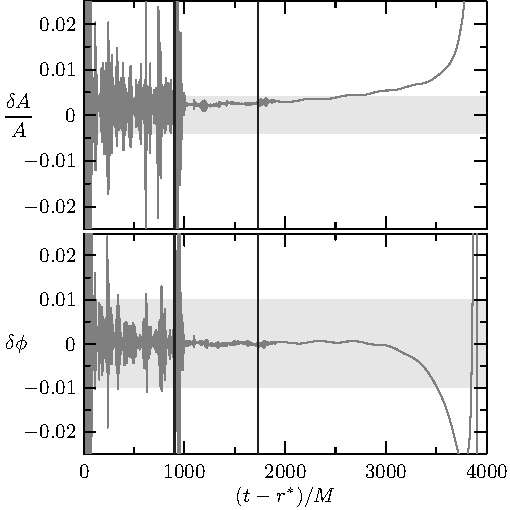
\includegraphics[width=0.55\linewidth]{figures/comparison/PlotDifferences}
%   \end{center}
%   \caption{Amplitude and phase differences between the numerical and
%     post-Newtonian waveforms, $\Psi_4$, that are blended to create the
%     hybrid waveform.  The vertical lines at $900M$ and $1730M$ denote
%     the region over which matching and hybridization occur.  Note that
%     the agreement is well within the numerical accuracy of the
%     simulation, represented by the horizontal bands, throughout the
%     matching region.  Also note that the phase difference is fairly
%     flat for a significant period of time after the matching range,
%     which indicates that the match is not sensitive to the particular
%     range chosen for matching.}
%   \label{fig:MatchingPhaseComparison}
% \end{figure}%
% %%%%%%%%%%%%%%%%%%%%%%%%%%%%%%%%%%%%%%%%%%%%%%%%%%%%%%%%%%%%%%%%%%%%%%
% In Fig.~\ref{fig:MatchingPhaseComparison} we compare the phase of the
% numerical and pN waveforms.  The quantities plotted are
% \begin{eqnarray}
%   \delta \phi & \equiv & \phi_{\pN} - \phi_{\NR}\ , \\
%   \frac{\delta A}{A} & \equiv & \frac{A_{\pN} - A_{\NR}}{A_{\NR}}\ , 
% \end{eqnarray}
% shown over the interval on which both data sets exist.  The vertical
% bars denote the matching region.  Note that the phase difference is
% well within the accuracy of the simulation (about 0.01 radians,
% represented by the horizontal band) over a range extending later than
% the matching region.  Also, the difference between the two is fairly
% flat, which implies that the match is not very sensitive to the region
% chosen for matching.  Because of this, we expect that the phase
% coherence between the early pN data and the late NR data will be
% physically accurate to high precision.
% 
% The hybrid waveform is then constructed by blending the two matched
% waveforms together according to
% \begin{eqnarray}
%   \label{eq:HybridWaveform}
%   A_{\hyb}(t) &= & \tau(t)\, A_{\NR} + \left[ 1 - \tau(t) \right]\,
%   A_{\pN}(t)\ , \\
%   \phi_{\hyb}(t) &= & \tau(t)\, \phi_{\NR} + \left[ 1 - \tau(t)
%   \right]\, \phi_{\pN}(t)\ .
% \end{eqnarray}
% The blending function $\tau$ is defined by
% 
% \begin{equation}
%   \label{eq:BlendingFunction}
%   \tau(t) = \left\{\begin{array}{ll}
%       0 & \mathrm{if}\quad t<t_{1}  \\
%       \frac{t-t_{1}}{t_{2}-t_{1}} & \mathrm{if}\quad t_{1} \leq t < t_{2} \\
%       1 & \mathrm{if}\quad t_{2} \leq t
%     \end{array} \right.
% \end{equation}
% 
% The values of $t_{1}$ and $t_{2}$ are the same as those used for the
% matching.  The amplitude discrepancy between the pN waveform and the
% NR waveform over this interval is within numerical
% uncertainty---roughly $0.4\%$.  As with the matching technique
% (Eq.~(\ref{eq:MatchingChiSquared})), this method is similar to that of
% Ref.~\cite{Ajith-Babak-Chen-etal:2007b}, but distinct, in that we
% blend the phase and amplitude, rather than the real and imaginary
% parts.  This leads to a smoothly blended waveform, shown in
% Fig~\ref{fig:WaveformSnapshot}.
% %%%%%%%%%%%%%%%%%%%%%%%%%%%%%%%%%%%%%%%%%%%%%%%%%%%%%%%%%%%%%%%%%%%%%%
% \begin{figure}
%   \begin{center}
%     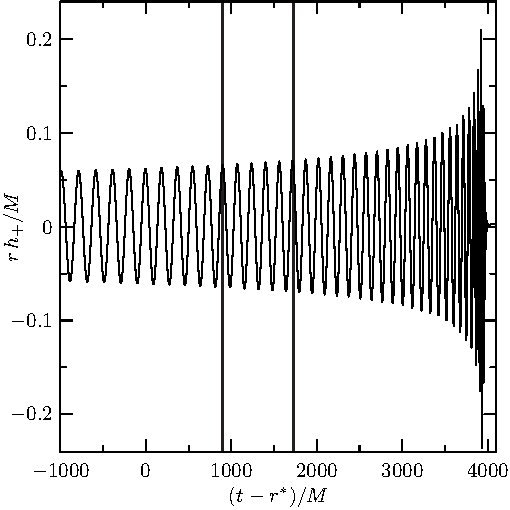
\includegraphics[width=0.55\linewidth]{figures/comparison/Waveform}
%   \end{center}
%   \caption{The last $t=5000\MSun$ of the hybrid waveform used in this
%     analysis: the $h_{+}$ waveform seen by an observer on the positive
%     $z$ axis.  The vertical lines denote the matching and
%     hybridization region.  The $0$ on the time axis corresponds to the
%     beginning of data from the numerical simulation.}
%   \label{fig:WaveformSnapshot}
% \end{figure}%
% %%%%%%%%%%%%%%%%%%%%%%%%%%%%%%%%%%%%%%%%%%%%%%%%%%%%%%%%%%%%%%%%%%%%%%
% 
% Up to this point, the waveform has been $\Psi_{4}$ data.  With the
% long waveform in hand, we numerically integrate twice to obtain $h$,
% and set the four integration constants so that the final waveform has
% zero average and first moment~\cite{Pfeiffer-Brown-etal:2007}.
% Because of the very long duration of the waveforms, this gives a
% reasonable result, which is only incorrect at very low
% frequencies---lower than any frequency of interest to us.  We have
% also checked that our results do not change when we effectively
% integrate in the frequency domain by taking
% \begin{equation}
%   \label{eq:PsiFourIntegration}
%   \tilde{h} = -\frac{\tilde{\Psi}_{4}}{4\,\pi\, f^{2}}\ ,
% \end{equation}
% which is the frequency-domain analog of the equation $\Psi_{4} =
% \ddot{h}$.
% \fi
% 
% 
% \section{Conclusions}
% 
% In this chapter we reviewed the basic properties of gravitational
% waves and methods used to model such waves from the inspiral and
% merger of systems of compact binaries.  In the next chapter we discuss
% the principles behind the LIGO detectors, which are looking for
% gravitational-wave signals.  Then in chapter~\ref{ch:search} we
% discuss how pN waveforms are used to detect signals in the LIGO data.
% 
% 
% % Todo:
% % Discuss the Weyl tensor, if needed for NR
